\documentclass[]{article}

\usepackage{graphicx}
\usepackage{listings}
\usepackage{color}
\usepackage{float}

\definecolor{mygray}{rgb}{0.4,0.4,0.4}
\definecolor{mygreen}{rgb}{0,0.8,0.6}
\definecolor{myorange}{rgb}{1.0,0.4,0}

\lstset{
	basicstyle=\footnotesize\sffamily\color{black},
	commentstyle=\color{mygray},
	frame=single,
	numbers=left,
	numbersep=5pt,
	numberstyle=\tiny\color{mygray},
	keywordstyle=\color{mygreen},
	showspaces=false,
	showstringspaces=false,
	stringstyle=\color{myorange},
	tabsize=2
}

% Title Page
\title{CAB301 Algorithms and Complexity}
\author{Nathan Perkins}


\begin{document}
\maketitle
\newpage
\tableofcontents
\newpage
\section{Executive Summary}
Bubble Sort is a historic sorting algorithm taught for its simplicity in design and operation. Analysis will be performed on the efficiency of the algorithm in respect to the swap flag improvement regarding the average case. 
\\\\
The analysis shows that the swap flag for the improved Bubble Sort performs better than the average case of the un-optimsed algorithm, however not to any appreciable degree. The swap flag improvement however, does increase performance when the array is already close to an ordered state. 
\section{Bubble Sort}
\subsection{Algorithm}
The general Bubble Sort algorithm works as follows. For every element in the array, successively compare each pair of adjacent elements, up until the total array size minus the current index, swapping each checked pair based on the comparison. For ascending sort, the comparison is if the previous element is larger than the next, and for descending sort the comparison is if the next element is larger than the previous. The reason that not all adjacent pairs are checked each iteration is due to the fact that for each iteration, the current highest element will shift to it's appropriate position in the array. For every iteration over the array size $n$, the ith element from the end of the listed is correctly indexed, and therefore no longer needs to be checked with further iterations. Appendix A lists the pseudo code example for the algorithm.
\subsection{Average Case Efficiency}
Due to the nature of the algorithm, iterating over the entire loop successively whilst check and swapping each adjacent pair, the algorithm is inefficient when compared to other methods of sorting. Bubble Sort has a computational efficiency on the order of $\mathcal{O}(n^2)$, with a more specific computational efficiency of $\frac{n^2}{2} + \frac{n}{2}$
\cite{BubbleSort}.
In contrast, more efficient algorithms like Heap Sort or Quick Sort have efficiencies on the order of $\mathcal{O}(n\log{}n)$,
which grows on a much slower scale than Bubble Sort \cite{HeapSort}.

\newpage

\section{Better Bubble Sort}
\subsection{Algorithm}
The basic Bubble Sort algorithm can be improved by introducing a swap flag. Without the swap flag, the algorithm will continue to compare elements of the array, regardless of whether the array has been sorted. A swap flag, which drives the main loop will ensure that the algorithm exits prematurely should the array elements reach a sorted state. Appendix A lists the better bubble sort algorithm using pseudo code.
\subsection{Basic Operation}
The operation chosen to analyse the efficiency of the algorithm is the comparison between array elements. In the case of the un-optimised algorithm, it will perform a number of comparisons equal to $\frac{n^2}{2} + \frac{n}{2}$, regardless of whether the array has been sorted. The optimised version has a chance to exit early if the array is sorted. Measuring the comparisons made is a good analytic. If the optimisation works as intended there should be less comparisons done, and overall an improvement in the design. 

\subsection{Average Case Efficiency}
The efficiency of the Better Bubble Sort algorithm is very similar to the original algorithms efficiency. It is of the same order as the original algorithm, as the fundamental design of its operation hasn't changed. However, the addition of the swap flag allows the algorithm to exit prematurely if it has completely sorted the array before the full algorithm has completed. Due to this check flag, it is very hard to quantify the improvements that this addition makes using theoretical analysis alone, as it is highly dependant on the ordering of the array given to the algorithm. Since the overall design of the algorithm hasn't significantly changed, it is expected that the general order of growth will be $\mathcal{O}(n^2)$, whilst it should be on average slightly faster than the original. 
\\\\
Constants are ignored when comparing efficiency and therefore two different algorithms can have the same order of growth, but still perform differently. The order of growth is calculated by examining the algorithm, which can be seen in Appendix A. This estimates the number of iterations required to reach completion. In Bubble sort, there are 2 defining loops which contribute to its efficiency. The outermost loop must iterate a number of times equal to the array size, whilst the innermost loop will similarly iterate a number of times equal to the array size minus the current index of the outer loop. Since the loops are embedded, the general order of magnitude is taken by multiplying both together, and only considering the highest power, results in the above efficiency. 
\section{Methodology}
\subsection{Computing Environment}
For experimental analysis, the computing environment can play a pivotal role in the specific results and has therefore been documented. 
\begin{enumerate}
	\item Operating System: The operating system used for the construction, data generation and analysis of report is Linux, specifically Ubuntu 15.10. This was chosen as it includes easy to use pre-installed packages that aid in the programming of C++ and python which was also used. All code was then checked to conform with Microsoft Windows for veracity of design.
	\item Algorithm: For creation of the algorithm, C++ was used. C++ is an efficient, and fast language that gives good freedom over design and memory, whilst still maintaining high level functionality. The Eclipse cross platform IDE was chosen to program the algorithm in, which gave access to debugging tools and automated compiling. For veracity, this was later ported to the code::blocks IDE and tested.
	\item Data Analysis
\begin{enumerate}
	\item Data types: Array size, number of iterations to sort the array, as well as time taken in seconds to complete are stored.
	\item Storage: CSV file format was used extensively to store the data directly via the C++ executable. CSV, or comma separated variables is an easy to use file format that separates all variables through the use of commas, this makes it perfect to easily get file formatting and output with C++. Python has in built functionality to interpret CSV files and was also a good choice in that regards, allowing the easy import of the data for plotting.
	\item Analysis: Python was used to interpret the data taken from CSV into graphs using the matplotlib graphing library. Python is a cross platform, high level scripting language with lots of in built scientific analysis features and is therefore a good choice to evaluate the data from any location or machine. matplotlib is a free library that easily plots data. 
\end{enumerate}
	\item Report: To build the report and everything included, LaTeX was used. LaTex allows good control over document flow and it's primary purpose, the easy inclusion of mathematical formulae and equations fits perfectly with the overall design of the report.
\end{enumerate}
\subsection{Test Data Generation}
To test the algorithm, it is important to note the types of arrays used as an input. Arrays sorted in specific manners can skew results, and lead to different performance than intended. As the main test of the report is on the average case, the generation of randomised arrays was of utmost importance. However, for testing the best case and worst case array generation was also created. 

\begin{enumerate}
	\item Random arrays: Initialising the random seed based on the current system time, then generating each element as a random number from 1-100. With each element being a random number with no association to the previous or next element, a truly randomised list is created.
	\item Ordered arrays: Initialising the random seed based on the current system time, setting the first element to be 1 and then proceeding to generate a random number between 0-9. It is then added to the previous array element and the next element is set equal to the result, ensuring that a strictly ascending array is generated. This is repeated until array size $n$.
	\item Reversed arrays: Initialising the random seed based on the current system time, setting the last element to be 1 and then proceeding to generate a random number between 0-9 and adding it to the next array element and setting the previous element equal to the result ensure that a strictly descending array is generated.
	\item Data Generation: The data for the overall testing is generated sequentially with increasing array sizes, repeated a number of times and then the average for that array size is then checked for validity and saved to the CSV. Data can then be presented as a continuous graph. Number of repeated operations was chosen as 100, and the array sizes saved are between $2\le n < 2000$
\end{enumerate}
\section{Implementation}
\subsection{Program}
The Bubble Sort algorithm is implemented in C++, and can be seen in Appendix B. As mentioned in the methodology section, randomised arrays were created and then sorted, counting the number of swap operations. Appendix B lists the code used to generate an array, as well as the functional code to generate an ascending order of increasing size(n) arrays. The function \textit{srand} was initialised in main, instead of the \textit{GenerateArray} function, to avoid problems with same seed timing issues.
\\\\
The main function instantiates a number of required variables, including file names, steps, duration, maximum array size and number of times to repeat. It then proceeds to generate random arrays up to the maximum size, and repeating to get the average of each array size. It then returns that average for both number of steps, representing computational operations, and the time taken for each sorting. This can be seen in Appendix B, the main function.

\subsection{Testing}
For testing purposes, a helper function was used throughout the whole development process, as well as actively being used in the data generation in the main function. IsSorted, as seen in Appendix B takes an array and checks if it's correctly sorted in ascending order. 
\\\\
For validity and checking purposes, reversed arrays and ordered arrays are also generated and compared against their theoretical results, these functions are also seen in Appendix B.
\section{Experimental Results}
\subsection{Operational Efficiency}
An addition has been made to the algorithm through the usage of num\_steps variable which keeps track of the number of swaps made and is incremented on the inner most loop, corresponding to each time an array swap has occurred. This can be seen in the comments of the code in Appendix B. The addition of the variable doesn't affect the overall performance in regards to growth of operational complexity. It has only a trivial affect on the duration for each iteration of the algorithm as it's only a single instruction addition.
\\\\
Comparing against the average case efficiency of the base algorithm, it can be seen in Appendix C that the swap flag version of the algorithm is remarkably similar for average case efficiency. With completely random arrays, it is expected that the array contains unsorted elements until the end and thus the average case efficiency hasn't improved significantly. There is some measurable difference between the two algorithms, as seen in Appendix C, however the difference is not significant.  
\\\\
To compare further against the un-optimised algorithm, the very worst case was computed for the optimised algorithm. The worst case for the optimised algorithm is when the swap flag gets no opportunity to exit prematurely. This will be when the array is completely reversed. Data was again generated as per the methodology section, with incremental array sizes from 2 to 2000, and the average of 100 cases per array size was taken. Results can be seen in Appendix C, The worst case for the optimised version is the same number of computations for the un-optimised average case. 
\\\\
The best case was also analysed. In the un-optimised bubble sort this is the same as the worst and average cases as the algorithm has no opportunity to exit early. As seen in appendix C, the optimised version of the algorithm has a linear order of growth. 

\subsection{Time Efficiency}
Time taken for each iteration was measured, repeated and then averaged as specified in implementation. Lines 43-45 in Appendix B, Main Function show the implementation of the timing function. Line 53 outlines the averaging of the data. The time taken measures the average execution time of the algorithm for that particular array size.
\\\\
The time taken is very similar to the order of growth on the computation steps. Both computation steps, as well as execution time are exponential growth algorithms and this can be seen in Appendix C, execution time for average case. Data ranges between 2 and 2000 size arrays, as specified in methodology. The time taken conforms to the expected results as computation steps and time taken are related, thus if the order of growth for computation is exponential, time taken must also be exponential. 
\\\\
To confirm results about the best case efficiency, when given a close to ordered array, time analysis was also performed on an ordered set of data. Seen in Appendix C - Ordered Execution time, the time taken grows only at a linear rate, due to the early exit. If the array is ordered it exits after a single pass.


\section{Appendix A - Algorithm}
The following is a pseudo code example of the non-optimized bubble sort algorithm. 
\begin{figure}[H]
	\caption{Basic Bubble Sort}
	\label{BasicBubbleSort}
\begin{lstlisting}[language=c++]
func bubblesort( var a as array )
	for i from 1 to length(a)
		for j from 0 to length(a) - i
			if a[j] > a[j + 1]
				swap( a[j], a[j + 1] )
end func
\end{lstlisting}
\end{figure}
The improved version of the Algorithm, listed below, adds in a swap flag which enables the function to exit prematurely should no swaps be made over an entire iteration of the outer loop.

\begin{figure}[H]\label{BetterBubbleSort}
	\caption{Improved Bubble Sort}
\begin{lstlisting}[language=c++]
func bubblesort( var a as array )
	bool swapped = true
	count = length(a)
	while (swapped)
		swapped = false
		for j from 0 to length(a) - count
			if a[j] > a[j + 1]
				swap( a[j], a[j + 1] )
				swapped = true
		count = count - 1
end func
\end{lstlisting}
\end{figure}
\section{Appendix B - C++ Implementation}
The algorithm below shows the improved Bubble Sort algorithm. num\_steps was added to the algorithm and returned, to indicate the number of computational steps taken. 
\begin{figure}[H]\label{BetterBubbleSortImplemented}
	\caption{Better Bubble Sort C++ Implementation}
	\begin{lstlisting}[language=c++]

int BetterBubbleSort(int array[], int size){
	int num_steps = 0; // This tracks the operation count
	int count = size-1;
	bool sflag = true;
	while (sflag){
		sflag = false;
		for (int j = 0; j<=count-1;j++){
			if (array[j+1] < array[j]){
				//Swap the 2 array elements
				int temp = array[j];
				array[j] = array[j+1];
				array[j+1] = temp;
				sflag = true;
			}
			num_steps++; //Increment the operation counter 
			//to indicate a comparison has been made			
		}
		count--;
	}
return num_steps; //Return the operation count
}
	\end{lstlisting}
\end{figure}
The arrays were generated with each element being a completely random variable to better simulate the natural state of an array during computation, as seen below. 
\begin{figure}[H]\label{SrandImp}
	\caption{Random Array Generation}
	\begin{lstlisting}[language=c++]
	int main() {
	
		srand(time(NULL));
		...
	}
	...
	void GenerateArray(int array[], int size){
		for(int i = 0; i<size;i++){
			int temp = rand()%100+1;
			array[i] = temp;
		}
	}
	\end{lstlisting}
\end{figure}
Seen below is the Main function for generating data. For each size of the array, i, it repeats the process a number of times based on the repeat variable. It then generates a random array, starts a timing function, sorts the array and then returns the time taken and number of steps. It then checks if the array is sorted and saves the average of the full averaged data. It then repeats the exact sequence for reversed and ordered arrays for checking and validity purposes, not included here for space.
\begin{figure}[H]\label{MainFunc}
	\caption{Main Function}
	\begin{lstlisting}[language=c++]
//================================================================
// Name        : BetterBubbleSort.cpp
// Author      : Nathan Perkins
// Version     :
// Copyright   : No Copyright
// Description : Better Bubble Sort in C++, Ansi-style
//================================================================

#include <iostream>
#include <stdlib.h>
#include <time.h>
#include <fstream>

using namespace std;

int BetterBubbleSort(int array[], int size);
bool IsSorted(int array[],int size);
void SortedPrint(int array[], int size);
void PrintArray(int array[], int size);
void GenerateArray(int array[], int size);
void GenerateOrderedArray(int array[],int size);
void GenerateReversedArray(int array[], int size);
bool SaveData(int num, int n, double time, char filename[]);

int main() {
	srand(time(NULL));
	int size = 2000;
	int repeat = 100;
	int steps;
	clock_t start;
	double duration;
	int i = 2;
	char filename[] = "BubbleSort.csv";
	char filename1[] = "BubbleSortOrdered.csv";
	char filename2[] = "BubbleSortReversed.csv";
	
	while (i<size){
		steps = 0;
		duration = 0.0;
		for(int j = 0;j<repeat;j++){
			int array[i];
			GenerateArray(array,i);
			start=clock();
			steps += BetterBubbleSort(array,i);
			duration += ( clock() - start)/(double) CLOCKS_PER_SEC;
			if(IsSorted(array,i)){
				if(j==0){
					cout<<"Iteration "<< i << " sorted"<< endl;
				}
			}
		}
		steps = steps/repeat;
		duration = duration/(double)repeat;
		if(!SaveData(steps,i,duration, filename)){
			cout<<"Writing to file failed:"<<endl;
			cout<<"Number: "<<i<<endl;
			cout<<"Steps:  "<<steps<<endl;
			cout<<"Time:   "<<duration<<endl;
			break;
		}
		i++;
	}
	cout<<"Finished Writing Random to file"<<endl;
	...
}
	\end{lstlisting}
\end{figure}
A function was defined to check if the array was correctly sorted, for use during testing, as well as during the full data implementation to check integrity of data.
\begin{figure}[H]\label{IsSorted}
	\caption{Checking if Array is sorted}
	\begin{lstlisting}[language=c++]
	bool IsSorted(int array[], int size){
		for(int i=1;i<size;i++){
			if(array[i]<array[i-1]){
				return false;
			}
		}
		return true;
	}
	\end{lstlisting}
\end{figure}
Listed below is the implementation of creating an ordered array, and also creating a completely reversed array.
\begin{figure}[H]\label{ReversedOrdered}
	\caption{Reversed and Ordered Array Generation}
	\begin{lstlisting}[language=c++]
	void GenerateOrderedArray(int array[], int size){
		array[0] = 1;
		for(int i = 1; i<size;i++){
			int temp = rand()%10+array[i-1];
			array[i] = temp;
		}
	}
	void GenerateReversedArray(int array[], int size){
		array[size-1] = 1;
		for(int i = size-2; i>=0;i--){
			int temp = rand()%10+array[i+1];
			array[i] = temp;
		}
	}
	\end{lstlisting}
\end{figure}
\section{Appendix C - Experimental Results}
As array size (n) increases, as seen below, it can be seen that the measured computational steps increases at a slower rate than $\frac{n^2}{2}$, denoted by the light blue line. 
\begin{figure}[H]\label{MeasuredRandom}
	\centering
	\caption{Bubblesort Operation Comparison: Expected vs Actual}
	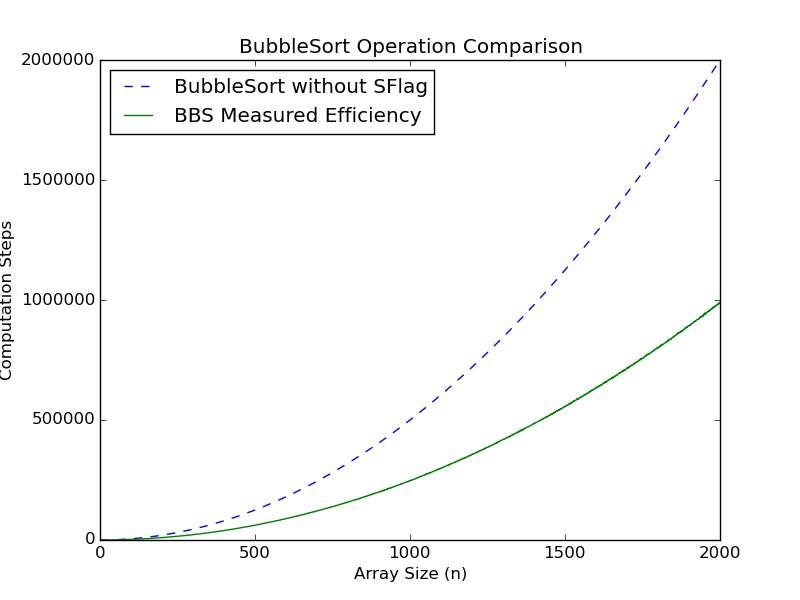
\includegraphics[width=0.8\textwidth]{Random.png}
\end{figure}
As the measured, and calculated average are too closely plotted together as seen above, the graph was zoomed at the end to show the discrepancy between calculated and measured. 
\begin{figure}[H]\label{MeasuredRandomZoom}
	\centering
	\caption{Bubblesort Operation Comparison: Expected vs Actual Zoomed}
	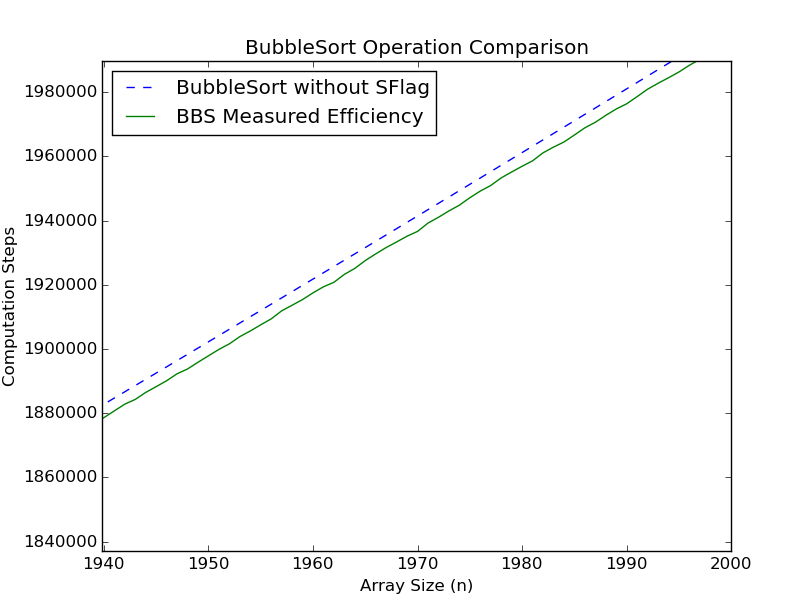
\includegraphics[width=0.8\textwidth]{RandomZoom.png}
\end{figure}
Computation steps for random array and reversed are very similar, due to the random distribution of elements within a random array, it is the case that the algorithm will not often get a chance to exit early.
\begin{figure}[H]\label{MeasuredReversed}
	\centering
	\caption{Bubblesort Reversed Array against average case}
	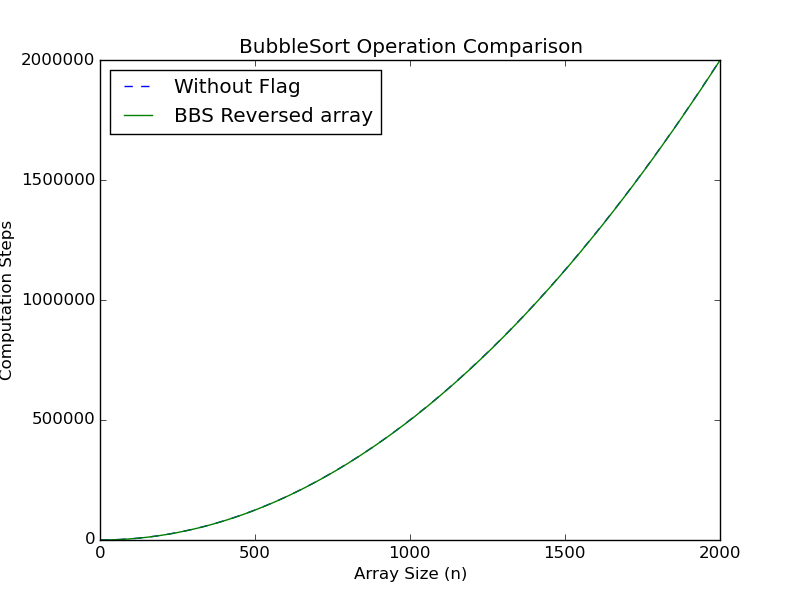
\includegraphics[width=0.8\textwidth]{Reversed.png}
\end{figure}
Ordered data was also tested, and as the graph was insignificant in comparison to the random array, it was instead plotted against the Heap Sort efficiency of $nlog(n)$. As can be seen below, ordered efficiency is on a linear growth order and much faster than even Heap Sort.
\begin{figure}[H]\label{MeasuredOrdered}
	\centering
	\caption{Bubblesort Ordered vs nlog(n)}
	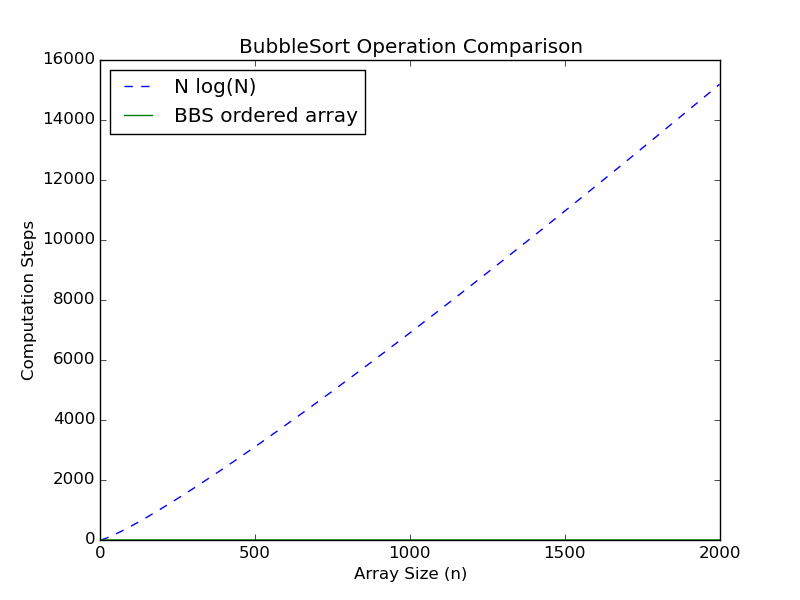
\includegraphics[width=0.8\textwidth]{Ordered.png}
\end{figure}
Execution time of Bubble sort with random arrays were also measured, as can be seen below, the data approximates an exponential growth order, with some data points rising higher than that. Likely those extreme points are due to the nature of using a non-RTOS, with system calls and other things interrupting the processor. Both the input and output data has been normalised to allow easier inference.
\begin{figure}[H]\label{MeasuredTime}
	\centering
	\caption{Bubblesort Execution Time - Average}
	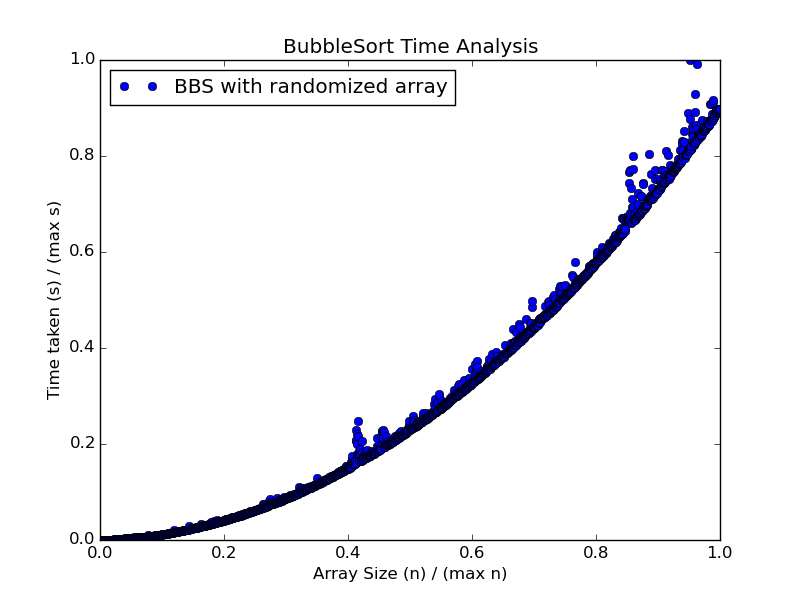
\includegraphics[width=0.8\textwidth]{RandomTime.png}
\end{figure}
Ordered data was also measured. Similar to the above diagram, some data points are skewed above the general trend for the same reasons. Both the input and output data has been normalised to allow easier inference.
\begin{figure}[H]\label{MeasuredTimeOrdered}
	\centering
	\caption{Bubblesort Execution Time - Ordered}
	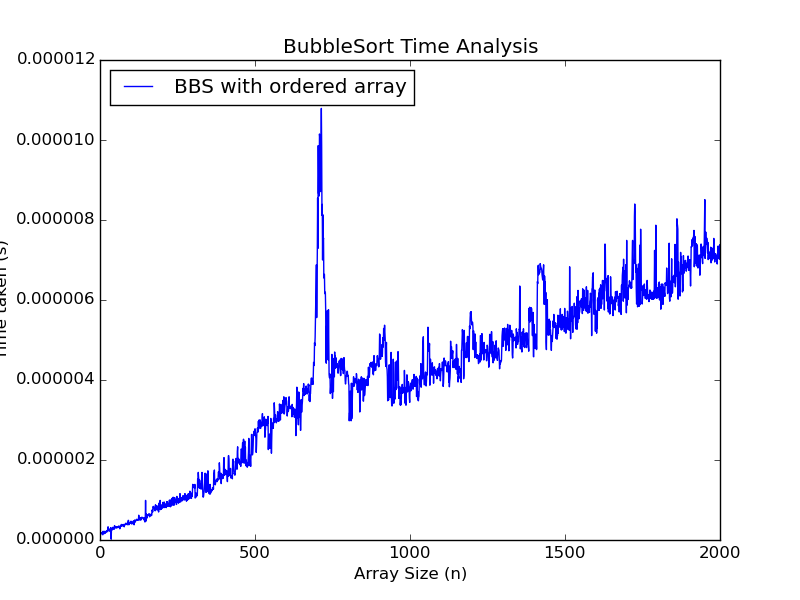
\includegraphics[width=0.8\textwidth]{OrderedTime.png}
\end{figure}
\bibliographystyle{IEEEtran}
\bibliography{References/FullRef}

\end{document}          
